\documentclass{beamer}
\usepackage[utf8]{inputenc}
\usepackage{tikz}
\usetikzlibrary{arrows.meta}
\tikzset{>={Latex[width=2mm,length=2mm]},
  base/.style = {
    rectangle, rounded corners, draw=black,
    minimum height=1cm, text centered, font=\sffamily
  },
  process/.style = {
    base, minimum width=2.5cm, fill=orange!15,
    font=\ttfamily
  },
}

\graphicspath{{./img/},{../2020_03/img/}}
\DeclareGraphicsExtensions{.png,.jpg,.pdf}

\usepackage{hyperref}
\hypersetup{colorlinks,urlcolor=blue!50!black,linkcolor=red}

\usepackage{fontawesome}
\usepackage{listings}

\title{\small Máster en Sistemas Electrónicos Avanzados (MSEA)\\\Large Co-simulación y verificación funcional con\\VHDL, C/C++ y Python/m\\{\small $\{$other$\}$}}
\author{Unai Martinez Corral\\\href{mailto:unai.martinezcorral@ehu.eus}{\faEnvelope~unai.martinezcorral@ehu.eus} ~\href{https://github.com/umarcor}{\faGithub~umarcor} ~\href{https://gitlab.com/umarcor}{\faGitlab~umarcor}}
\institute{Escuela de Ingeniería de Bilbao\\Universidad del País Vasco/Euskal Herriko Unibertsitatea (UPV/EHU)}
\date{2021/05}

\begin{document}

\frame{\titlepage}

\begin{frame}
\frametitle{Other open source projects}
\begin{minipage}[t]{.495\linewidth}
Project management:
\begin{itemize}
  \item tsfpga
  \href{https://gitlab.com/truestream/tsfpga}{\faGit} \href{https://truestream.gitlab.io/tsfpga/}{\faBook}
  \href{https://pypi.org/project/tsfpga/}{\faCode}

  \item fusesoc
  \href{https://github.com/olofk/fusesoc}{\faGithub}
  \href{https://fusesoc.rtfd.io/}{\faBook}
  \href{https://pypi.org/project/fusesoc/}{\faCode}

  \item edalize
  \href{https://github.com/olofk/edalize}{\faGithub}
  \href{https://edalize.rtfd.io}{\faBook}
  \href{https://pypi.org/project/edalize/}{\faCode}

  \item litex
  \href{https://github.com/enjoy-digital/litex}{\faGithub}

  \item duh
  \href{https://github.com/sifive/duh}{\faGithub}
\end{itemize}
\vspace{1em}

Waveform viewer/drawer:
\begin{itemize}
  \item wavedrom
  \href{https://github.com/wavedrom/wavedrom}{\faGithub}
  \href{https://wavedrom.com/}{\faGlobe}
\end{itemize}
\end{minipage}
\begin{minipage}[t]{.49\linewidth}
Android:
\begin{itemize}
  \item termux \href{https://termux.com/}{\faGlobe} \href{https://github.com/termux}{\faGithub}
  \begin{itemize}
      \item gcc\_termux \href{https://github.com/its-pointless/gcc_termux}{\faGithub}
  \end{itemize}
\end{itemize}
\vspace{1em}

Formal verification:
\begin{itemize}
  \item ghdlsynth-beta
  \href{https://github.com/tgingold/ghdlsynth-beta}{\faGithub}

  \item yosys
  \href{https://github.com/YosysHQ/yosys}{\faGithub}
  \href{http://www.clifford.at/yosys/}{\faGlobe}

  \item nextpnr
  \href{https://github.com/YosysHQ/nextpnr}{\faGithub}

  \item SymbiYosys
  \href{https://github.com/YosysHQ/SymbiYosys}{\faGithub}
  \href{https://symbiyosys.rtfd.io}{\faBook}
\end{itemize}
\end{minipage}
\end{frame}

\begin{frame}
\frametitle{SymbiFlow}
\centering
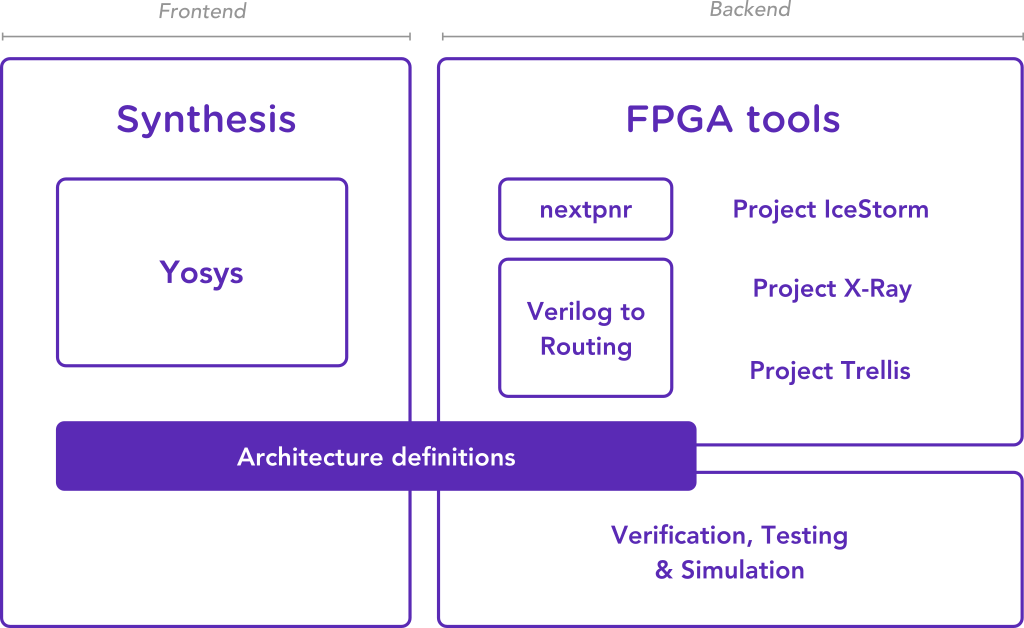
\includegraphics[width=\linewidth]{symbiflow.png}
\vfill
\Large\href{https://symbiflow.github.io/}{symbiflow.github.io}
\end{frame}

\end{document}

